%-------------------------------------------------------------------------------
%	PACKAGES AND OTHER DOCUMENT CONFIGURATIONS
%-------------------------------------------------------------------------------
\documentclass{article}% A4 paper and 11pt font size

\usepackage{amsmath,amsfonts,amsthm} % Math packages
\usepackage{graphicx}
\usepackage{float}
\usepackage{caption}
\usepackage{subcaption}
\usepackage{fullpage}
\usepackage{url}
%-------------------------------------------------------------------------------
%	TITLE SECTION
%-------------------------------------------------------------------------------

\title{
\textsc{Neural Networks} \\ [25pt]
\huge ANN Project Report \\ % The assignment title
}

\author{Adam Swart} % Your name

\date{\today} % Today's date or a custom date

%%%%%%%%%%%%%%%%%%%%%%%%%%%%%%%%%%%%%%%%%%%%%%%%%%%%%%%%%%%%%%%%%%%%%%%
%DOCUMENT
%%%%%%%%%%%%%%%%%%%%%%%%%%%%%%%%%%%%%%%%%%%%%%%%%%%%%%%%%%%%%%%%%%%%%%%
\begin{document}
\maketitle % Print the title
%%%%%%%%%%%%%%%%%%%%%%%%%%%%%%%%%%%%%%%%%%%%%%%%%%%%%%%%%%%%%%%%%%%%%%%
\section{Introduction}
Neural Networks are constructed and trained for each of the following data sets, each of which was obtained from \url{https://archive.ics.uci.edu/ml/datasets.html}. The same approach is used for each neural network: import and normalise the data; partition the data into a training set, a test set, and a validation set; and find the optimum training algorithm through a process of trial and error. Each neural network's degree of fit is assessed, and performance is analysed using the MATLAB postregression function.

\section{Wine} 
The wine dataset is the result of a chemical analysis of wines taken from three different cultivars from the same region in Italy. There are $13$ attributes for each instance, and each attribute is a real value. The attributes are: alcohol, malic acid, ash, alcalinity of ash, magnesium, total phenols, flavanoids, nonflavanoid phenols, proanthocyanins, colour intensity, hue, OD280/OD315 of diluted wines, and proline. 
\\
Our first step is to import the data from the text file. No normalisation or encoding is necessary since all the input patterns are real numbers and the targets are integers. We construct a feed-forward network with $2$ layers, each layer with $5$ neurons. We find that with the Levenburg-Marquardt backpropagation with $1000$ epochs and the maximum number of failed validations set to $20$, the minimum gradient is found quickly (after $49$ iterations). We partition the data set into a training set, test set, and validation set, and begin training.

\begin{figure}[H]
\centering
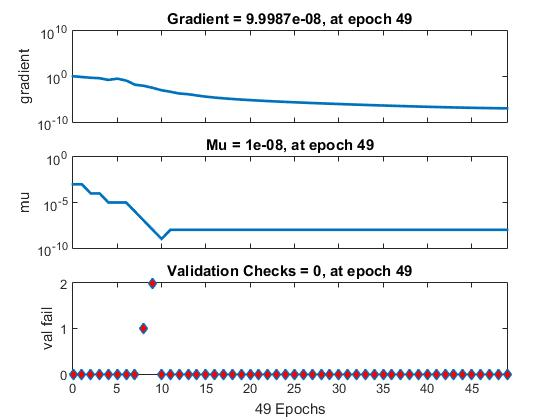
\includegraphics[scale=0.5]{Wine/train_state.jpg}
\caption{Wine train state.}
\label{fig:winetrain}
\end{figure}
\\
Once training is finished, we save all variables. We are now ready to test the network. On the training set, the correlation coefficient is $0.999995$ and the $r^2$ value is $0.999989$. On the test set, the correlation coefficient is $0.960454$ and the $r^2$ value is $0.913144$. On the entire data set, the correlation coefficient is $0.98618$ and the $r^2$ value is $0.971409$. This indicates a high degree of accuracy. The postregression values were $0.999854$, $1.00324$, and $1.00132$ for the training set, test set, and entire set respectively.
\begin{figure}[H]
\centering
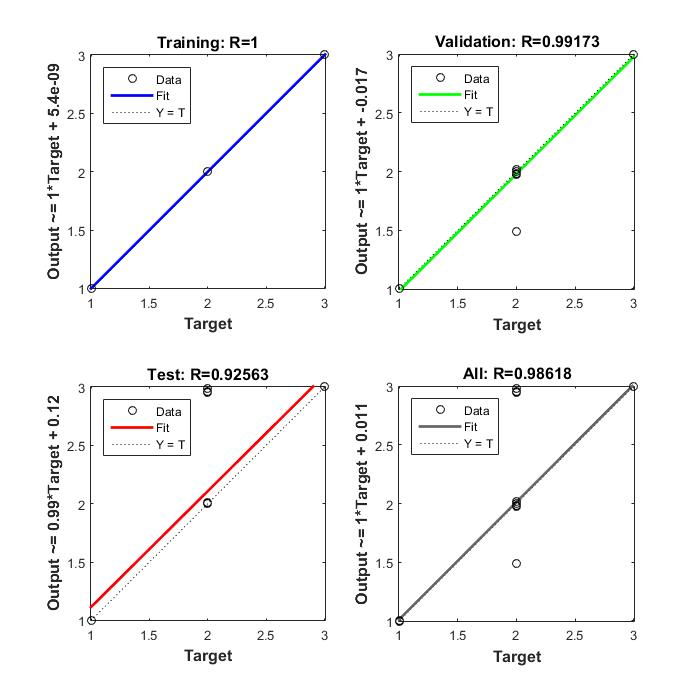
\includegraphics[scale=0.3]{Wine/regression.jpg}
\caption{Wine neural network training regression.}
\label{fig:winereg}
\end{figure}
\\
The degree of fit of the network is highly accurate. The network trains well on the data and reaches a minimum error quickly.

\section{Mushrooms}
The mushroom dataset includes descriptions of hypothetical samples of $23$ species of gilled mushroom in the Agaricus and Lepiota family. Each sample is classified as either edible or poisonous, and has $22$ attributes. Each attribute can be one of several letters indicating the value of the attribute.
\\
We import and encode the data. Since each attribute is a lower case letter, we convert the attribute to its ASCII value and subtract $97$. Now if any attribute is less than $0$ we know that this instance has a missing entry.
\\
We construct a 2-layer feed-forward network. The first layer has $20$ neurons and the second layer has $10$ neurons. Since this is a relatively large dataset we choose the scaled conjugate gradient backpropagation algorithm with $1000$ epochs and the maximum number of failed validations set to $20$. We partition the data into a training set, a test set, and a validation set. We train the network.
\begin{figure}[H]
\centering
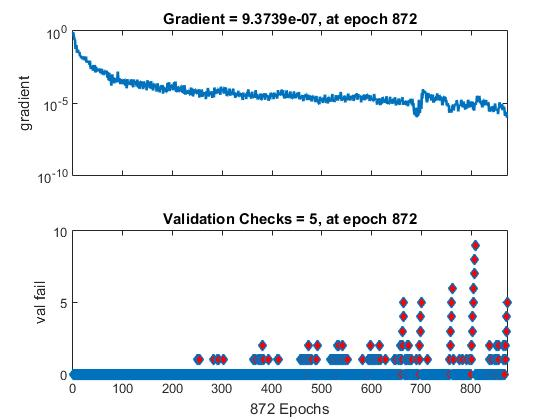
\includegraphics[scale=0.5]{Mushrooms/train_state.jpg}
\caption{Mushrooms train state.}
\label{fig:mushtrain}
\end{figure}
\\
We find that the network converges to the minimum gradient close to the maximum number of epochs. Once training is complete we save all variables and begin testing. We find that on the training set, the test set, and the entire set, the correlation coefficient is $1$ and the $r^2$ value is $1$. The postregression value is $1$, $0.999996$, and $1$ for the training set, test set, and whole set respectively. This indicates an optimal degree of fit.
\begin{figure}[H]
\centering
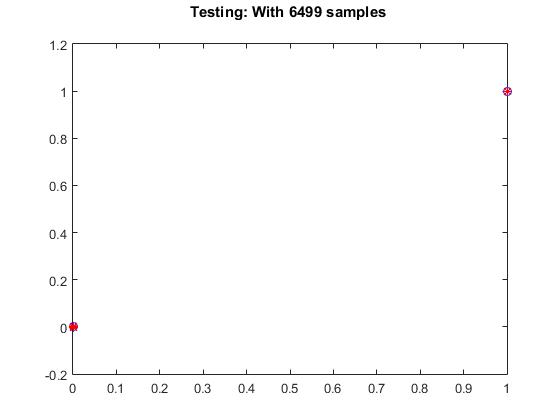
\includegraphics[scale=0.3]{Mushrooms/testing.jpg}
\caption{Mushrooms testing. Activations and targets match.}
\label{fig:mushtest}
\end{figure}


\section{Iris}
The iris dataset contains $3$ classes, each of $50$ instances. Each instance has $4$ attributes: sepal length in centimetres, sepal width in centimetres, petal length in centimetres, and petal width in centimetres. The classes are Iris-Setosa, Iris-Versicolour, and  Iris-Virginica. 
\\
We import the data and encode the targets: we set Iris-Setosa, Iris-Versicolour, and  Iris-Virginica to $0$, $1$, and $2$ respectively. We construct a 2-layer feed forward neural network, each layer with 10 neurons. We use the scaled conjugate gradient backpropagation algorithm with $1000$ epochs and the maximum number of failed validations set to $20$. We partition the data into a training set, a test set, and a validation set. We train the network.
\begin{figure}[H]
\centering
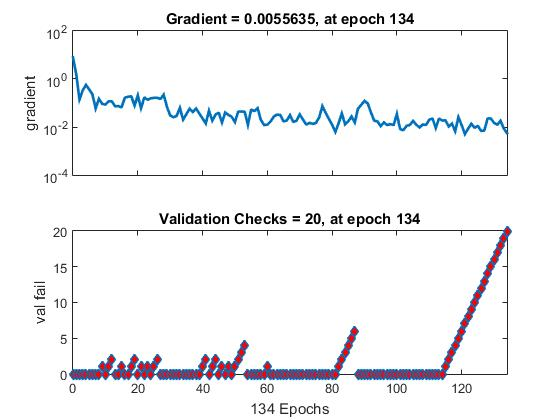
\includegraphics[scale=0.5]{Iris/train_state.jpg}
\caption{Iris train state.}
\label{fig:iristrain}
\end{figure}
\\
The maximum number of failed validations is exceeded and training ceases. We save all variables and begin testing. On the training set, the correlation coefficient is $0.983743$ and the $r^2$ value is $0.966971$. On the test set, the correlation coefficient is $0.995552$ and the $r^2$ value is $0.990767$. On the entire data set, the correlation coefficient is $0.984217$ and the $r^2$ value is $0.968362$. The postregression values were $0.950495$, $0.986778$, and $0.958892$ for the training set, test set, and entire set respectively.
\begin{figure}[H]
\centering
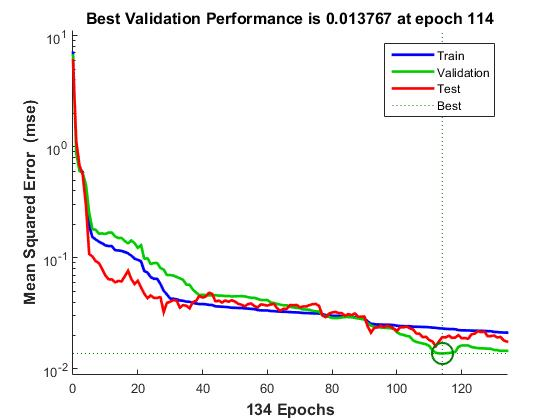
\includegraphics[scale=0.5]{Iris/performance.jpg}
\caption{Iris performance.}
\label{fig:iristrain}
\end{figure}
\\
While the postregression values, $r^2$ values, and correlation coefficients are not entirely optimal, the degree of fit is highly accurate.

\section{Abalone}
The abalone dataset predicts the age of abalone from 8 attributes. The dataset has 4177 instances.
\\
We import and normalise the data. We assign a value of $0$ for the Male attribute, $1$ for the Female attribute, and $2$ for the Infant attribute. We construct a 2-layer feed forward neural network, each layer with 15 neurons. We use the Polak-Ribiere conjugate gradient backpropagation algorithm with $1000$ epochs and the maximum number of failed validations set to $20$. We partition the data into a training set, a test set, and a validation set, and train the network.
\begin{figure}[H]
\centering
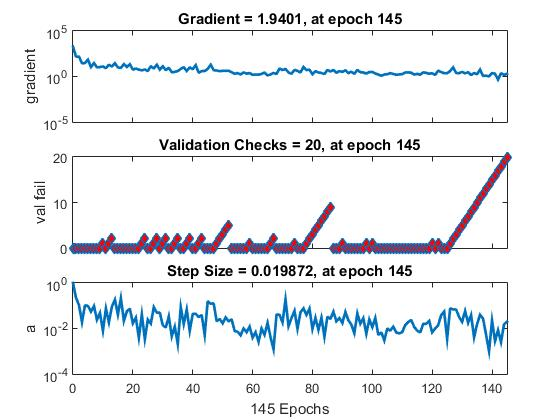
\includegraphics[scale=0.5]{Abalone/training.jpg}
\caption{Abalone training state.}
\label{fig:abtrain}
\end{figure}
The maximum number of failed validations is exceeded and training ceases. We save all variables and begin testing. On the training set, the correlation coefficient is $0.758545$ and the $r^2$ value is $0.574383$. On the test set, the correlation coefficient is $0.758359$ and the $r^2$ value is $0.574525$. On the entire data set, the correlation coefficient is $0.759644$ and the $r^2$ value is $0.57656$. The postregression values were $0.597163$, $0.586786$, and $0.594014$ for the training set, test set, and entire set respectively. This indicates a poor degree of fit. 
\begin{figure}[H]
\centering
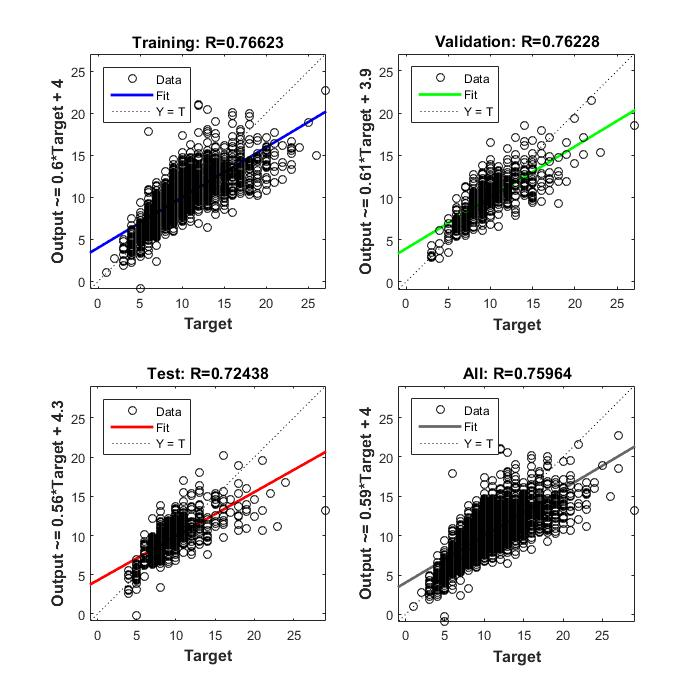
\includegraphics[scale=0.5]{Abalone/regression.jpg}
\caption{Abalone training regression.}
\label{fig:abtrain}
\end{figure}
The distribution of data makes it difficult to find an accurate degree of fit.

\section{Concrete}
The concrete benchmark dataset predicts the compressive strength of concrete given 8 quantitative inputs.
\\
We import the data. No normalisation or encoding is needed. We construct a 3-layer feed forward neural network, each layer with 20 neurons. We use the scaled conjugate gradient backpropagation algorithm with $1000$ epochs and the maximum number of failed validations set to $20$. We partition the data into a training set, a test set, and a validation set, and train the network.
\begin{figure}[H]
\centering
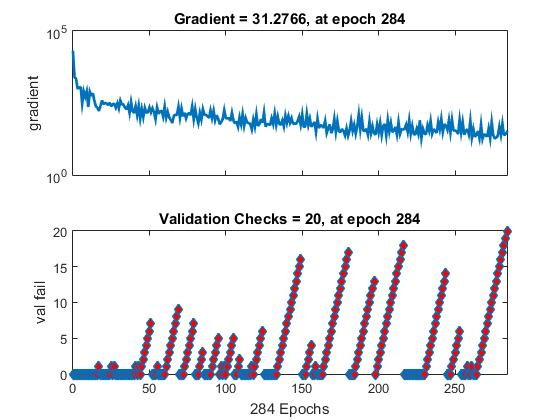
\includegraphics[scale=0.5]{Concrete/training.jpg}
\caption{Concrete training state.}
\label{fig:contrain}
\end{figure}
The maximum number of failed validations is exceeded and training ceases. We save all variables and begin testing. On the training set, the correlation coefficient is $0.960284$ and the $r^2$ value is $0.921712$. On the test set, the correlation coefficient is $0.950959$ and the $r^2$ value is $0.904218$. On the entire data set, the correlation coefficient is $0.958799$ and the $r^2$ value is $0.918972$. The postregression values were $0.942134$, $0.911618$, and $0.935799$ for the training set, test set, and entire set respectively. This indicates an accurate degree of fit. 
\begin{figure}[H]
\centering
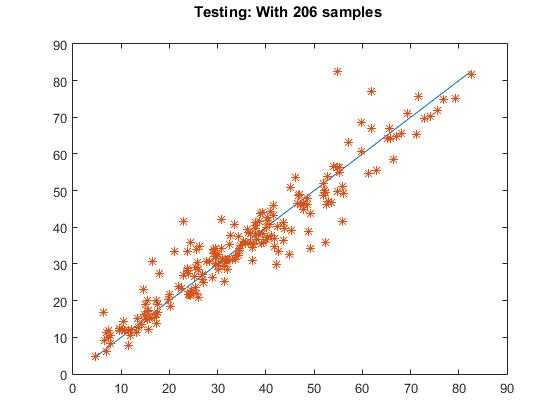
\includegraphics[scale=0.5]{Concrete/test.jpg}
\caption{Concrete degree of fit.}
\label{fig:conreg}
\end{figure}
The degree of fit, although not optimal, is accurate.

%%%%%%%%%%%%%%%%%%%%%%%%%%%%%%%%%%%%%%%%%%%%%%%%%%%%%%%%%%%%%%%%%%%%%%%
\end{document} 